\documentclass[main.tex]{subfiles}
\begin{document}

世界是多姿多彩的,而姿需图,彩即色.先说色.
“ 五颜六色”是一个汉语成语,形容色彩复杂或花样繁多,但数字5和6并无确切的含义.“ 五彩缤纷、万紫千红”里面的5、1,000和10,000也如此.但色彩需要数学来准确地描述.古人以最突出的七种颜色的合称“七彩”,则是确有所指,来自彩虹.
采用传统中国文化说法,毛泽东把它们写进了诗:“ 赤橙黄绿青蓝紫\footnote{赤橙黄绿青蓝紫: red, orange, yellow, green, cyan,blue, purple.},谁持彩练当空舞?”\footnote{《菩萨蛮·大柏地》}青色就是偏蓝的绿色。
考虑到匀称性以及物理学中对太阳光的光谱分析,科学说法则是红橙黄绿蓝靛紫\footnote{红橙黄绿蓝靛紫: red, orange, yellow, green, blue, indigo, purple.},
需要把蓝变深一点取代青,而且之后加上靛色.

770~622nm,感觉为红色;622~597nm,橙色;597~577nm,黄色;577~492nm,绿色;492~455nm,蓝靛色;455~390nm,紫色。

网络超文本标记语言HTML 支持 141 种颜色。用 Python 编程 SVG 生成的这些颜色图如 \ref{fig:1.4.2}.

\begin{figure}
	\centering
	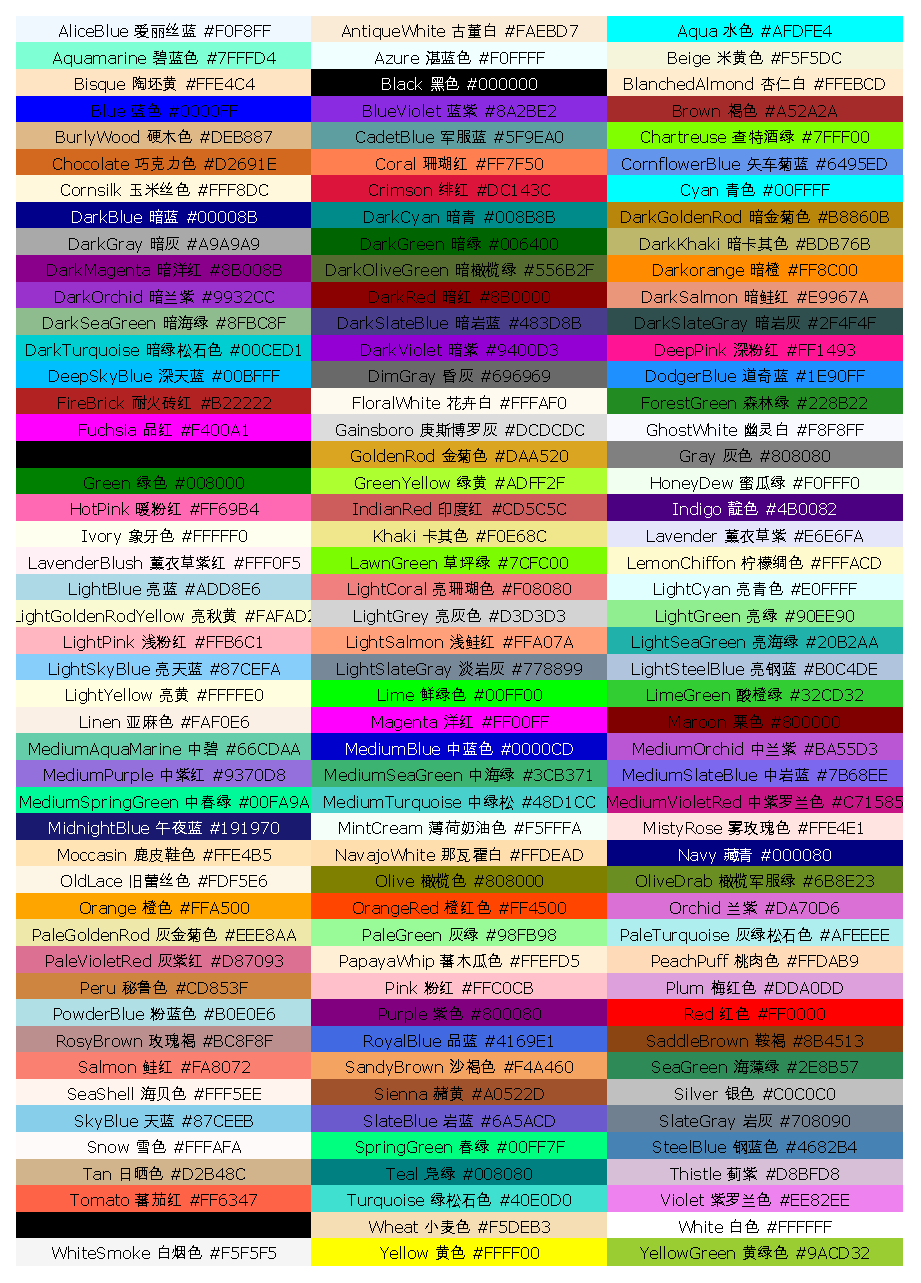
\includegraphics[width=1\columnwidth]{svg/html_colors.eps}
	\caption{HTML 支持的 141 种颜色}
	\label{fig:1.4.2}
\end{figure}
cyan = 1.0 - red

magenta = 1.0 - green

yellow = 1.0 - blue

indigo \#4B0082 75, 0, 130

\begin{figure}
	\centering
	
\includegraphics[width=0.5\columnwidth]{svg/simple_example.eps}
	\caption{简单例子}
	\label{fig:I.1.}
\end{figure}



爱丽丝蓝%#F0F8FF
古董白%#FAEBD7
水色%#00FFFF
海蓝宝石% #7FFFD4
天蓝色%#F0FFFF
米色% #F5F5DC
浓汤%#FFE4C4
\end{document} 
